%!TEX root = synthese.tex
\newpage
\section{Design Pattern - Proxy}

\subsection{Objectifs}

Les droits liés à l’ouverture d’une session ont un impact sur les commandes et traitements proposés. Dans cet incrément nous allons restreindre les accès à certaines commandes pour les utilisateurs. Les objectifs de l'incrément 6 sont les suivants :\\
\begin{itemize}
\item Lecture seule : Pas de modification des données des utilisateurs ls et cat sont autorisées;
\item Lecture/écriture : Les commandes mkdir, touch, ln et rm sont autorisées.\\
\end{itemize}

Pour cet incrément,  nous utiliserons le pattern Proxy. Le proxy joue le rôle d’un aiguilleur par rapport aux droits d’accès des utilisateurs. 

\subsection{Implémentation}

Pour chaque commande, il existe une classe proxy associée. L'UML suivant montre ce pattern uniquement avec la commande ls.

\begin{figure}[!h]
\centering
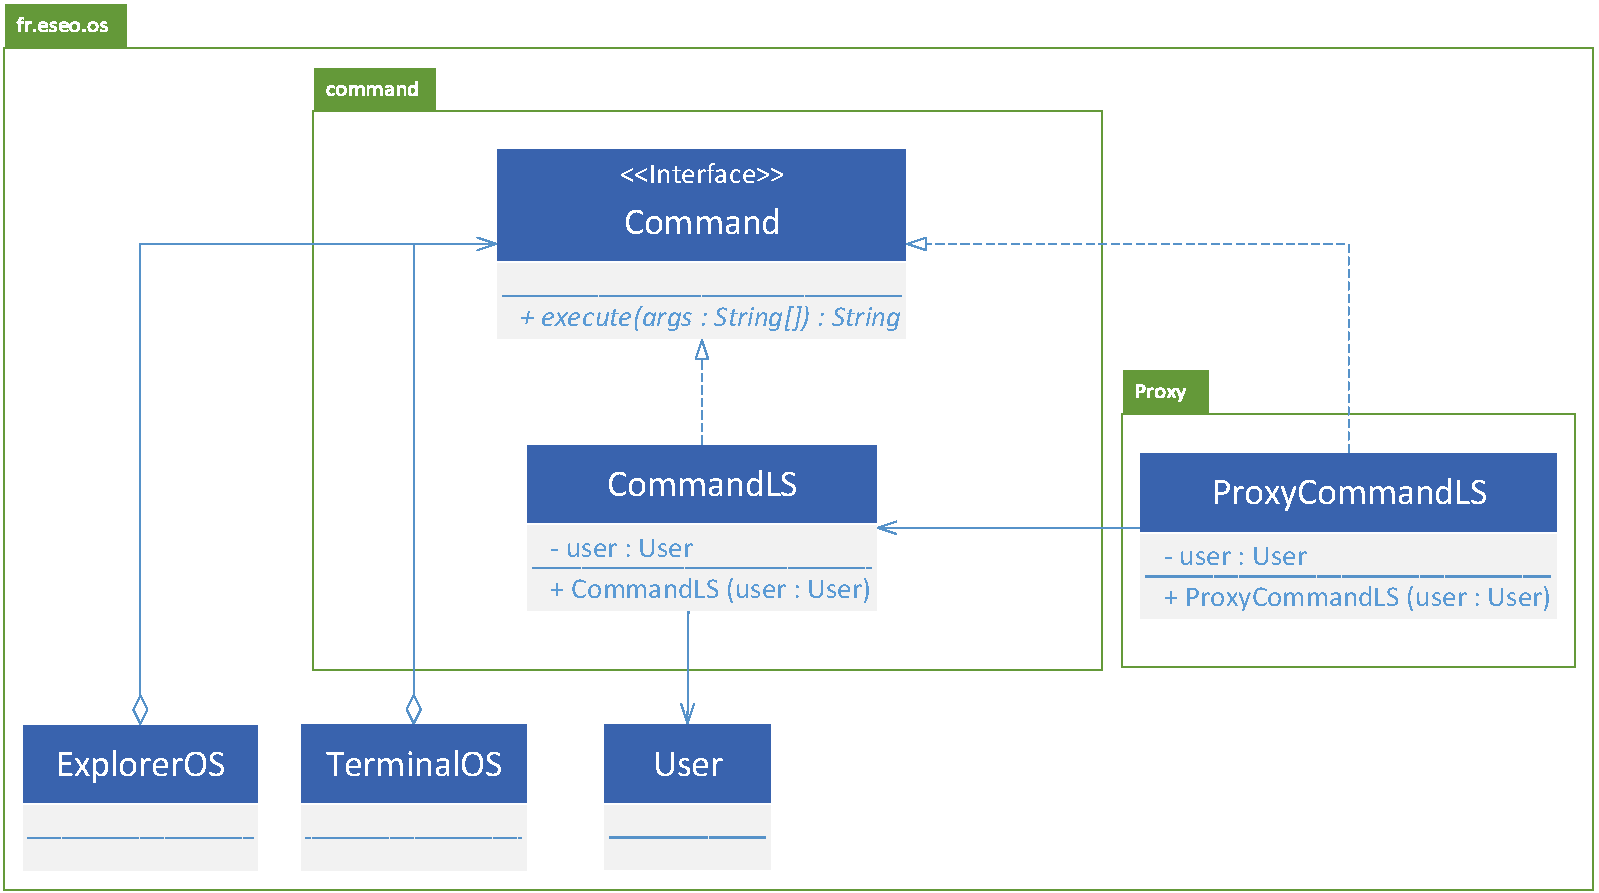
\includegraphics[width=\textwidth]{../uml/uml-proxy}
\end{figure}

Au lieu que le client (\emph{TerminalOS} et \emph{ExplorerOS}) appelle la commande directement, il va appeler le proxy associé. Ce proxy va vérifier si l'utilisateur a les accès (avec la méthode \emph{hasReadOnlyAccess()}) et va rediriger l'execution la commande. On a utilisé la commande touch comme exemple par la suite.

\begin{lstlisting}
package fr.eseo.os.command;
public class CommandTOUCH implements Command {

    private User user;

    public CommandTOUCH(User user) {
        this.user = user;
    }

    @Override
    public String execute(String... args) {
        return user.executeCommandTOUCH(args);
    }
}
\end{lstlisting}

Le proxy implémente la même interface que la commande associée.

\begin{lstlisting}
package fr.eseo.os.proxy;
public class ProxyCommandTOUCH implements Command {

    private User user;

    public ProxyCommandTOUCH(User user) {
        this.user = user;
    }

    @Override
    public String execute(String... args) {
        if (this.user.hasReadWriteAccess()) {
            Command commandTOUCH = new CommandTOUCH(user);
            return commandTOUCH.execute(args);
        } else {
            return AccessEnum.FORBIDDEN.getAccess();
        }
    }
}
\end{lstlisting}

Enfin, dans la classe \emph{TerminalOS}, on modifie le constructeur afin qu'on instancie le proxy plutôt que la commande. Ainsi, on ne modifie rien de plus dans le programme. La méthode \emph{runCommand} appelera maintenant le proxy.

\clearpage
\begin{lstlisting}

public TerminalOS(String login, String password, 
					String access){
	...

	this.commandLS = new ProxyCommandLS(this.user);
	this.commandCAT = new ProxyCommandCAT(this.user);
	this.commandTOUCH = new ProxyCommandTOUCH(this.user);
	this.commandRM = new ProxyCommandRM(this.user);
	this.commandMKDIR = new ProxyCommandMKDIR(this.user);
	this.commandLN = new ProxyCommandLN(this.user);

	...
}
\end{lstlisting}

